\documentclass{article}
\usepackage[a4paper]{geometry}
\usepackage{amsfonts}
\usepackage{alltt}
\usepackage{amsmath,amssymb}        % Mathpack für Formeln jeder Art
\usepackage[parfill]{parskip}       % Autoamtisch Newline, wenn Zeilenumbruch im Quelltext.
\usepackage[utf8]{inputenc}         % UTF8 Zeichensatz. 
\usepackage{xstring}				% Gebraucht für Circuitikz
\usepackage{tikz}                   % Wichtig für Zeichnungen aller Art
\input{kvmacros}                    % Kv Diagramme
\usepackage[siunitx]{circuitikz}    % Diagramme und Schaltungen
\usepackage{pgffor}
\usepackage{fancyhdr}
\usepackage{array}
\usepackage{fullpage}


\tikzstyle{help lines}=[blue!50,very thin]
\tikzstyle{help lines}+=[dashed]
\tikzstyle{Kreis}= [circle,draw]


\title{RS - Übung 9}
\author{Arne Beer (MN 6489196), \\
Rafael Epplee (MN 6269560), \\
Julian Polatynski (MN 6424884)}

\begin{document}
\maketitle



\section*{9.1}

	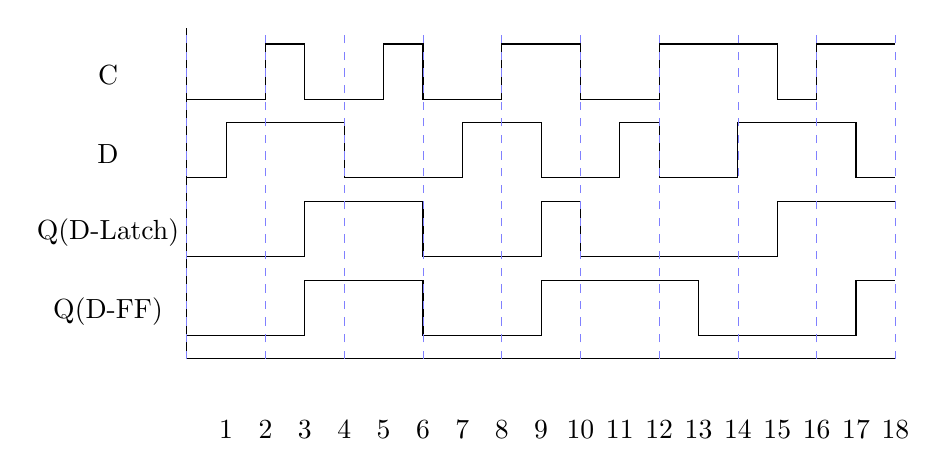
\begin{tikzpicture}
		\draw
			(1,0.4) -- (10,0.4) {}
	        (1,0.4) -- (1,4.6) {}

	        (1.5,-0.5) node[] {1}
	        (2,-0.5) node[] {2}
	        (2.5,-0.5) node[] {3}
	        (3,-0.5) node[] {4}
	        (3.5,-0.5) node[] {5}
	        (4,-0.5) node[] {6}
	        (4.5,-0.5) node[] {7}
	        (5,-0.5) node[] {8}
	        (5.5,-0.5) node[] {9}
	        (6,-0.5) node[] {10}
	        (6.5,-0.5) node[] {11}
	        (7,-0.5) node[] {12}
	        (7.5,-0.5) node[] {13}
	        (8,-0.5) node[] {14}
	        (8.5,-0.5) node[] {15}
	        (9,-0.5) node[] {16}
	        (9.5,-0.5) node[] {17}
	        (10,-0.5) node[] {18}

	        (0,4) node[] {C}
	        (0,3) node[] {D}
	        (0,2) node[] {Q(D-Latch)}
	        (0,1) node[] {Q(D-FF)}

	         (1,3.7) -- (2,3.7)-- (2,4.4) --(2.5,4.4) --(2.5,3.7) --(3.5,3.7) -- (3.5,4.4) --
	         (3.5,4.4) -- (4,4.4) -- (4,3.7) -- (5,3.7) -- (5,4.4) -- (6,4.4) -- (6,3.7) -- 
	         (7,3.7) -- (7,4.4) -- (8.5,4.4) -- (8.5,3.7) --(9,3.7) -- (9,4.4) -- (10,4.4)

	         (1,2.7) -- (1.5,2.7) -- (1.5,3.4) -- (3,3.4) -- (3,2.7) -- (4.5,2.7) -- (4.5,3.4) 
	    	 -- (5.5,3.4) -- (5.5,2.7) -- (6.5,2.7) -- (6.5,3.4) -- (7,3.4) -- (7,2.7) -- 
	    	 (8,2.7) -- (8,3.4) -- (9.5,3.4) -- (9.5,2.7) -- (10,2.7)

	    	 (1,1.7) -- (2.5,1.7) -- (2.5,2.4) -- (4,2.4) -- (4,1.7) -- (5.5,1.7) -- 
	    	 (5.5,2.4) -- (6,2.4) -- (6,1.7) -- (8.5,1.7) -- (8.5,2.4) -- (10,2.4) 

	    	 (1,0.7) -- (2.5,0.7) -- (2.5,1.4) -- (4,1.4) -- (4,0.7) -- (5.5,0.7) -- (5.5,1.4) --(7.5,1.4) -- (7.5,0.7) -- (8.5,0.7) -- (9.5,0.7) -- (9.5,1.4) -- (10,1.4)  
	    ;
	    \draw[style=help lines]
	    (1.0,0.4) grid (1.0,4.6)
	    (2.0,0.4) grid (2.0,4.6)
	    (3.0,0.4) grid (3.0,4.6)
	    (4.0,0.4) grid (4.0,4.6)
	    (5.0,0.4) grid (5.0,4.6)
	    (6.0,0.4) grid (6.0,4.6)
	    (7.0,0.4) grid (7.0,4.6)
	    (8.0,0.4) grid (8.0,4.6)
	    (9.0,0.4) grid (9.0,4.6)
	    (10.0,0.4) grid (10.0,4.6)

	    ;

        \end{tikzpicture}

\section*{9.2}

	\subsection*{a)}
	1. Flipflop mit Multiplexer \\

			\begin{tabular}{|c|c|c||c|}\hline
			D & E & CLK & $Q^+$ \\ \hline
			0 & 0 & 0 & Q \\
			0 & 0 & $\uparrow$ & Q \\
			0 & 1 & 0 & Q \\
			0 & 1 & $\uparrow$ & 0 \\
			1 & 0 & 0 & Q \\
			1 & 0 & $\uparrow$ & Q \\
			1 & 1 & 0 & Q \\
			1 & 1 & $\uparrow$ & 1 \\ \hline


		\end{tabular}\\
		\\

	2. Flipflop mit Taktausblendung \\

	\begin{tabular}{|c|c|c||c|}\hline
			D & E & CLK & $Q^+$ \\ \hline
			0 & 0 & 0 & Q \\
			0 & 0 & 1 & Q \\
			0 & 1 & 0 & Q \\
			0 & 1 & 1 & 0 \\
			1 & 0 & 0 & Q \\
			1 & 0 & 1 & Q \\
			1 & 1 & 0 & Q \\
			1 & 1 & 1 & 1 \\ \hline


		\end{tabular}


	\subsection*{b)}

	Beide Flipflops geben nur dann D weiter, wenn CLK=E=1 . Man könnte diese Schaltung also für Sicherungen benutzen. Die Idee ist, dass der Wert nur dann weitergegeben wird, wenn die Prüfsumme, in unserem Fall E, gesendet würde. Andernfalls würde das fehlerhafte D gesendet werden. 
	Auch könnte man dadurch erreichen, dass bei einem gleichmäßigen Takt bestimmt wird, an welchem Zeitpunkt D eingelesen wird. 

	\subsection*{c)}

	In der 1. Variante wird der Output des Flipflops zurück in den 2:1-Multiplexer geleitet. Dadurch wird bei jedem Takt, solange $E=0$ Der Ausgangswert des Flipflops erneut in diesen eingelesen. Im Falle, dass $E=1$ entsteht ein Hazard, da D erst über den Multiplexer zum Flipflop geleitet werden muss.

	In der 2. Variante hingegen sind E und CLK durch ein AND verknüpft. Hier wird das Taktsignal also nur gegeben, wenn E und CLK true sind. Außerdem entsteht auch hier beim verifizieren des Taktsignals ein statischer Hazard, sodass das Taktsignal um einen Takt verspätet ankommt. 

	Dadurch ist die 2. Variante nicht geeignet, da sie immer den Wert von D einliest, der einen Takt später gesendet wird. 
	Bei Variante 1 tritt ein statischer Hazard bei der Weiterleitung von D auf, wodurch immer der Wert von D gewählt wird, der einen Takt vor dem Taktsignal gesendet wurde. 


\section*{9.3}

	\subsection*{a)}

Zustandsdiagramm für die Ampel der Hauptstraße:\\
\\

	\begin{tikzpicture}[shorten >=2pt]



		\node [Kreis] (0) at (1.5,6) {$z_0$\ $000$};
		\node [Kreis] (1) at (2.5,2.75) {$z_1$};
		\node [Kreis] (2) at (6,1.5) {$z_2$};
		\node [Kreis] (3) at (9.5,2.75) {$z_3$};
		\node [Kreis] (4) at (10.5,6) {$z_4$};
		\node [Kreis] (5) at (9.5,9.5) {$z_5$};
		\node [Kreis] (6) at (6,10.5) {$z_6$};
		\node [Kreis] (7) at (2.5,9.5) {$z_7$};

		\draw[thick,->]
		(0) .. controls (1.5,4.0) .. (1);
		\draw[thick,->]
		(1) .. controls (4,1.5) .. (2);
		\draw[thick,->]
		(2) .. controls (7.8,1.5) .. (3);
		\draw[thick,->]
		(3) .. controls (10.5,4) .. (4);
		\draw[thick,->]
		(4) .. controls (10.5,8) .. (5);
		\draw[thick,->]
		(5) .. controls (7.8,10.5) .. (6);
		\draw[thick,->]
		(6) .. controls (4,10.5) .. (7);
		\draw[thick,->]
		(7) .. controls (1.5,8) .. (0);
		;


	\end{tikzpicture}\\



	\subsection*{b)}
	
	\begin{tabular}{|c|c| c c c || c c c | c c c | c c c |}\hline
		z & i & $z_2$ & $z_1$ & $z_0$ & $z_{2}^+$ & $z_{1}^+$ & $z_{0}^+$ & $rt_H$ & $ge_H$ & $gr_H$ & $rt_N$ & $ge_N$ & $gr_N$ \\ \hline

			$z_0$ & * & 0 & 0 & 0 & 0 & 0 & 1 &	1 & 0 & 0 & 1 & 0 & 0\\
			$z_1$ & * & 0 & 0 & 1 & 0 & 1 & 0 & 1 & 1 & 0 & 1 & 0 & 0\\
			$z_2$ & 0 & 0 & 1 & 0 & 0 & 1 & 0 & 0 & 0 & 1 & 1 & 0 & 0\\
			$z_2$ & 1 & 0 & 1 & 0 & 0 & 1 & 1 & 0 & 0 & 1 & 1 & 0 & 0\\
			$z_3$ & * & 0 & 1 & 1 & 1 & 0 & 0 & 0 & 1 & 0 & 1 & 0 & 0\\
			$z_4$ & * & 1 & 0 & 0 & 1 & 0 & 1 & 1 & 0 & 0 & 1 & 0 & 0\\
			$z_5$ & * & 1 & 0 & 1 & 1 & 1 & 0 & 1 & 0 & 0 & 1 & 1 & 0\\
			$z_6$ & * & 1 & 1 & 0 & 1 & 1 & 1 & 1 & 0 & 0 & 0 & 0 & 1\\
			$z_7$ & * & 1 & 1 & 1 & 0 & 0 & 0 & 1 & 0 & 0 & 0 & 1 & 0\\ \hline



	\end{tabular}


	\subsection*{c)}


	Kv-Diagramm für $rt_H$:

	\karnaughmap{3}{$f:$}{{$z_1$}{$z_2$}{$z_0$}}{11110011}{}
	{
	\put(-2,0.5){\oval(3.9,0.8)[]}
	\put(-3,1){\oval(1.9,1.9)[]}
	}\\
\\
DNF: $z_2\vee \overline{z_1}$\\

---------------------------------

	Kv-Diagramm für $ge_H$:

	\karnaughmap{3}{$f:$}{{$z_1$}{$z_2$}{$z_0$}}{010001000}{}
	{
	\put(-2,1.5){\oval(1.9,0.9)[]}
	}\\
\\
DNF: $z_0\wedge\overline{z_2}$\\

---------------------------------

	Kv-Diagramm für $gr_H$:

	\karnaughmap{3}{$f:$}{{$z_1$}{$z_2$}{$z_0$}}{000010000}{}
	{
	\put(-0.5,1.5){\oval(0.9,0.9)[]}
	}\\
\\
DNF: $\overline{z_2}\wedge\overline{z_1}\wedge\overline{z_0}$\\

---------------------------------

	Kv-Diagramm für $rt_N$:
	
	\karnaughmap{3}{$f:$}{{$z_1$}{$z_2$}{$z_0$}}{11111100}{}
	{
	\put(-3,1){\oval(1.9,1.9)[]}
	\put(-2,1.5){\oval(3.9,0.8)[]}
	}\\
\\
DNF: $\overline{z_2}\vee \overline{z_1}$\\

---------------------------------

	Kv-Diagramm für $ge_N$:
	
	\karnaughmap{3}{$f:$}{{$z_1$}{$z_2$}{$z_0$}}{00010001}{}
	{
	\put(-2,0.5){\oval(1.9,0.8)[]}
	}\\
\\
DNF: $z_2\wedge z_0$\\


	Kv-Diagramm für $gr_N$:


	\karnaughmap{3}{$f:$}{{$z_1$}{$z_2$}{$z_0$}}{00000010}{}
	{
	\put(-0.5,0.5){\oval(0.9,0.9)[]}
	}\\
\\
DNF: $z_2\wedge z_1\wedge\overline{z_0}$\\

---------------------------------

	Kv-Diagramm für $z^+_2$:

	\karnaughmap{3}{$f:$}{{$z_1$}{$z_2$}{$z_0$}}{00110110}{}
	{
	\put(-3,0.5){\oval(1.9,0.8)[]}
	\put(0,0.5){\oval(1.9,0.9)[l]}
	\put(-4,0.5){\oval(1.9,0.9)[r]}
	}\\
\\
DNF: $(z_2\wedge\overline{z_1})\vee (z_2\wedge \overline{z_0})\vee(z_0\wedge z_1\wedge \overline{z_2})$\\

---------------------------------

		Kv-Diagramm für $z^+_1$:

	\karnaughmap{3}{$f:$}{{$z_1$}{$z_2$}{$z_0$}}{01011010}{}
	{
	\put(-0.5,1){\oval(0.9,1.9)[]}
	\put(-2.5,1){\oval(0.9,1.9)[]}
	}\\
\\
DNF: $(z_0\wedge \overline{z_1})\vee (z_1\wedge \overline{z_0})$\\

---------------------------------

		Kv-Diagramm für $z^+_0$:

	\karnaughmap{3}{$f:$}{{$z_1$}{$z_2$}{$z_0$}}{00101010}{}
	{
	\put(0,0.5){\oval(1.9,0.8)[l]}
	\put(-4,0.5){\oval(1.9,0.8)[r]}
	\put(-0.5,1){\oval(0.9,1.9){}}
	}\\
\\
DNF: $(z_1\wedge \overline{z_0})\vee (z_2\wedge \overline{z_0})$\\




	\end{document}

